\chapter{Grammaires locales}
\label{chap-grammars}

Les grammaires locales sont un moyen puissant de représenter la plupart des phéno-
mènes linguistiques. La première section présentera le formalisme sur lesquel ces
grammaires reposent. Nous verrons ensuite comment construire et présenter des grammaires
avec Unitex.


\section{Formalisme des grammaires locales}
\index{Grammaires!formalisme}

\subsection{Grammaires algébriques}
Les grammaires Unitex sont des variantes des grammaires algébriques, également appelées
grammaires hors-contexte.\index{Grammaires!context-free} Une grammaire algébrique est constituée de
règles de réécriture. Voici une grammaire qui reconnaît n’importe quel nombre de caractères $a$:

\bigskip $S \rightarrow$ $aS$

$S \rightarrow$ \E

\bigskip
\noindent Les symboles figurant à gauche des règles sont appelés \textit{symboles
 non-terminaux}\index{Symboles!non-terminaux}\index{Symboles non-terminaux}                                                                                       car ils peuvent être réécrits. Les symboles qui ne peuvent pas être réécrits par des règles sont
 appelés \textit{symboles terminaux}\index{Symboles!terminaux}. Les membres droits des règles
sont des suites de symboles non-terminaux et terminaux. Le symbole epsilon noté \E ~
désigne le mot vide. Dans la grammaire ci-dessus, $S$ est un symbole non-terminal et
$a$ un terminal. $S$ peut se réécrire soit en un $a$ suivi d’un $S$,
soit en mot vide. L’opération de réécriture par l’application d’une règle est appelée
\textit{dérivation}.\index{Dérivation} On dit qu’une grammaire reconnaît un mot s’il existe
une suite de dérivations qui produit ce mot. Le non-terminal qui sert de point de départ
à la première dérivation est appelé \textit{axiome}.\index{Axiome}\index{Règles!réécriture}


\bigskip
\noindent La grammaire ci-dessus reconnaît ainsi le mot \textit{aa}, car on peut obtenir ce
mot depuis l’axiome $S$ en effectuant les dérivations suivantes:

\bigskip Dérivation 1: réécriture de l’axiome en $aS$

\underline{$S$} $\rightarrow aS$

\bigskip Dérivation 2: réécriture du $S$ du membre droit en $aS$

$S$ $\rightarrow a$\underline{$S$} $\rightarrow aaS$

\bigskip Dérivation 3: réécriture du $S$ to \E

$S$ $\rightarrow aS \rightarrow aa$\underline{$S$} $\rightarrow aa$

\bigskip
\noindent On appelle \textit{langage d’une grammaire} l’ensemble des mots reconnus par celle-ci.
%\textit{languagegenerated by the grammar}.
Les langages reconnus par les grammaires algébriques sont appelés \textit{Languages algébriques}
\index{Langages algébriques} ou \textit{Langages hors-contexte}\index{Langages hors-contexte}.


\subsection{Grammaires algébriques étendues}
\index{Grammaires!algébriques étendues}

   Les grammaires algébriques étendues sont des grammaires algébriques où les membres
droits des règles ne sont plus des suites de symboles mais des expressions rationnelles.
\index{Expressions rationnelles} Ainsi, la grammaire reconnaissant une suite quelconque de $a$
peut se réécrire en une grammaire étendue d’une seule règle:


\bigskip $S \rightarrow$ $a^{*}$

\bigskip
\noindent Ces grammaires, également appelées \textit{réseaux de transitions récursifs}
(\textit{RTN en Anglais})\index{Recursive Transition Networks}\index{RTN} ou
\textit{diagrammes de syntaxe}\index{Diagrammes de syntaxe}, se prêtent à une représentation graphique
conviviale. En effet, le membre droit d’une règle peut être représenté par un graphe dont le nom
est le membre gauche de la règle.


\bigskip
\noindent Toutefois, les grammaires Unitex ne sont pas exactement des grammaires algébriques
étendues, car elles intégrent la notion de \textit{transduction}.\index{Transduction} Cette notion,
empruntée aux automates à états finis, signifie qu’une grammaire peut produire des sorties.
Dans un souci de clarté, nous utiliserons malgré tout les termes grammaire ou graphe.
Quand une grammaire produira des sorties, nous utiliserons le terme \textit{transducteur},
\index{Transducteur} par extension de la définition d’un transducteur dans le domaine des automates
à états finis.\index{Automates!à états finis}


\section{Édition de graphes}
\label{section-editing-graphs}

\subsection{Création d'un graphe}
Pour pouvoir utiliser des graphes Intex dans Unitex, il faut les convertir en Unicode. Le
procédé de conversion est le même que pour les textes (voir section~\ref{fig-new-graph}).
Le symbole en forme de flèche est \textit{l'état initial} du graphe.\index{Etat!initial} Le symbole
composé d'un rond contenant un carré est  \textit{l'état final} du graphe.\index{Etat!final} La
grammaire reconnaît les séquences décrites par les chemins allant de l'état initial à l'état final


\begin{figure}[!h]
\begin{center}
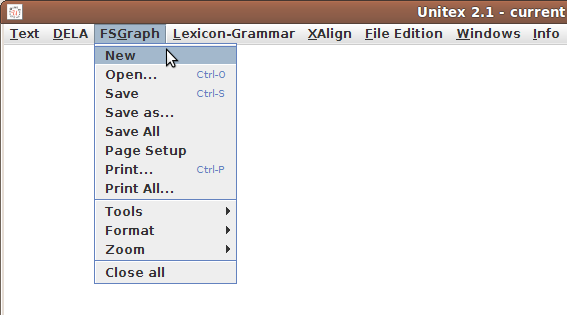
\includegraphics[width=13cm]{resources/img/fig5-1.png}
\caption{Menu FSGraph}
\end{center}
\end{figure}

\begin{figure}[!h]
\begin{center}
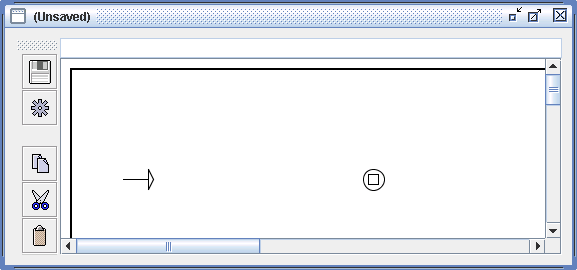
\includegraphics[width=14.5cm]{resources/img/fig5-2.png}
\caption{Graphe vierge\label{fig-new-graph}}
\end{center}
\end{figure}

\bigskip
\noindent Pour créer une boîte, cliquez sur la fenêtre tout en appuyant sur la touche Ctrl. 
\index{Graphe!création d'une boîte} \index{Création d'une boîte}\index{Boîtes!création}
Vous verrez alors apparaître un carré bleu symbolisant la boîte vide créée (voir figure
~\ref{fig-box-creation}). Lors de la création d’une boîte, celle-ci est automatiquement sélectionnée.


\bigskip
\noindent Vous voyez donc le contenu de la boîte s’afficher dans la zone de texte située en
haut de la fenêtre. La boîte créée contient le symbole \verb+<E>+\index{\verb+<E>+} qui représente
le mot vide epsilon. Remplacez ce symbole par le texte \verb$I+you+he+she+it+we+they$ et validez en
appuyant sur la touche Entrée. Vous venez de créer une boîte contenant sept lignes (voir
	figure~\ref{fig-pronoun-box}).
En effet, le caractère \verb$+$ sert de séparateur.\index{\verb$+$} La boîte apparaît sous la
forme de lignes de texte rouge car elle n’est pour l’instant reliée à aucune autre.
On utilise souvent ce type de boîtes pour insérer des commentaires dans un graphe.
\index{Graphe!commentaires}\index{Commentaires!dans un graphe}

\bigskip
\noindent Si vous souhaitez ajouter un commentaire dans un graphe, vous devez créer une boîte qui
commence par \verb$/$. Le texte de la boîte est affiché en vert, et peut contenir des lignes vides.
La boîte ne peut avoir, ni de transition entrante, ni de transition sortante (voir
	figure~\ref{comment-box}).

\begin{figure}[!h]
\begin{center}
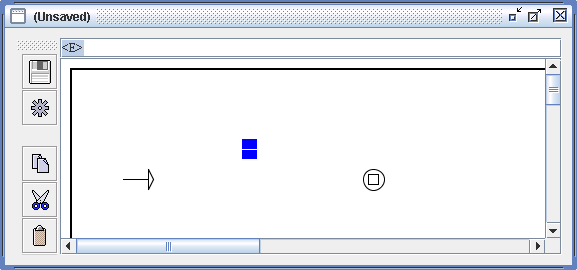
\includegraphics[width=14.5cm]{resources/img/fig5-3.png}
\caption{Création d’une boîte\label{fig-box-creation}}
\end{center}
\end{figure}

\begin{figure}[!h]
\begin{center}
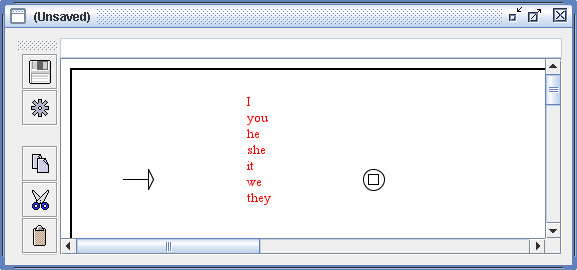
\includegraphics[width=14.5cm]{resources/img/fig5-4.png}
\caption{Boîte contenant
\texttt{I+you+he+she+it+we+they}\label{fig-pronoun-box}}
\end{center}
\end{figure}

\begin{figure}[!h]
\begin{center}
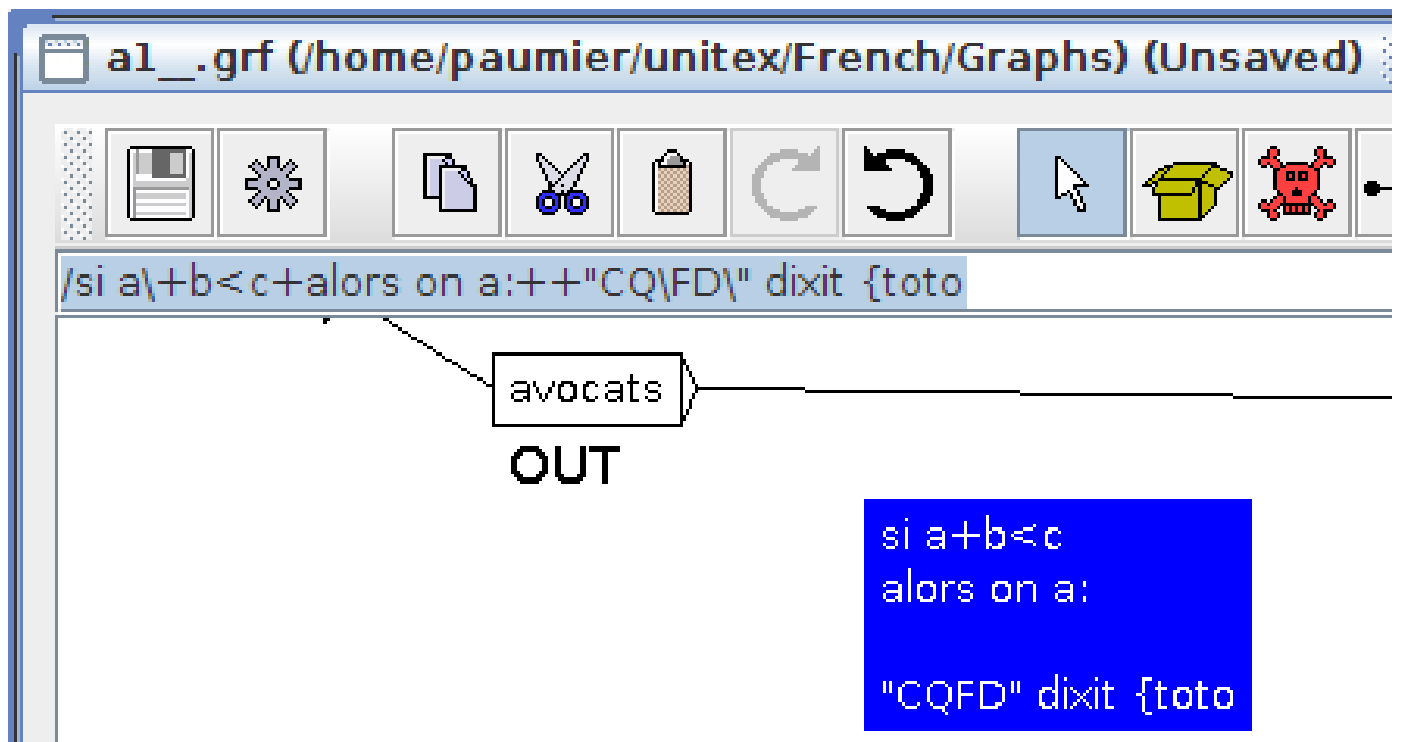
\includegraphics[width=12.5cm]{resources/img/fig5-4b.png}
\caption{Boîte contenant un commentaire\label{comment-box}}
\end{center}
\end{figure}
%\clearpage


%\clearpage
\noindent Pour relier une boîte à une autre, il faut cliquer sur la boîte de départ, puis sur la
boîte de destination.\index{Graphe!connexion des boîtes}\index{Boîtes!connexion}
S’il y a déjà une transition entre les deux boîtes, celle-ci est enlevée. Il est possible
d’effectuer cette même opération en cliquant d’abord sur la boîte de destination, puis sur la boîte
de départ tout en pressant sur la touche Shift.
Dans notre exemple, une fois la boîte reliée à l’état initial et à l’état final du graphe,
on obtient le graphe de la figure~\ref{fig-pronoun-graph}:

\begin{figure}[!ht]
\begin{center}
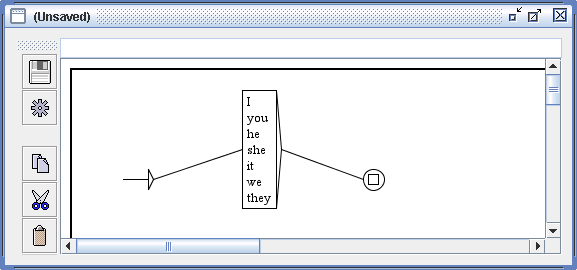
\includegraphics[width=14.5cm]{resources/img/fig5-5.png}
\caption{Graphe reconnaissant des pronoms anglais\label{fig-pronoun-graph}}
\end{center}
\end{figure}

\bigskip
\noindent REMAQUE: si vous double-cliquez sur une boîte, vous relierez cette boîte à elle-même (voir
figure~\ref{fig-loop-box}). Pour annuler, double-cliquez une nouvelle fois sur la boîte.

\bigskip
\begin{figure}[!h]
\begin{center}
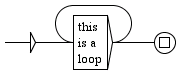
\includegraphics[width=4.5cm]{resources/img/fig5-6.png}
\caption{Boîte reliée à elle-même\label{fig-loop-box}}
\end{center}
\end{figure}

\noindent Cliquez sur "Save as..." dans le menu "FSGraph" pour enregistrer le graphe
\index{Graphe!enregistrement}. Par défaut, Unitex propose d'enregistrer le graphe dans le 
sous-répertpoire \verb+Graphs+ de votre répertoire personnel. Vous pouvez voir si le graphe a été
modifié après le dernièr enregistrement  en vérifiant si le titre du graphe contient le texte
\verb+(Unsaved)+.


%%%%%%%%%%%%%%%%%%%%%%%
\bigskip
\noindent Lorsque vous modifiez un graphe, vous pouvez faire apparaître, par un clic droit, un menu
contextuel vous permettant d'effectuer les opérations les plus usuelles.

\begin{itemize}
\item création d'une boîte
\item enregistrement, impression du graphe courant ou modifier les paramètres de la page
\item les menus habituels "Tools", "Format" et "Zoom" également accessibles dans le menu "FSGraph"
\end{itemize}
Si une ou plusieurs boîtes sont sélectionnées, les menus suivants deviennent accessibles, et
permettent d'effectuer plusieurs types d'opérations sur cet ensemble de boîtes. Sinon, ils sont
inutiles et donc désactivés. 
\begin{itemize}
\item entourer les boîtes sélectionnées avec des variables normales, des varaiables de sorties, des
contextes, ou des délimiteurs du mode morphologique. Ces opérations sont également réalisables avec
la barre d'outils de la fenêtre d'édition du graphe (voir section~\ref{toolbar-commands}). 
\item fusionner les boîtes sélectionnées
\item exporter les boîtes sélectionnées en tant que nouveau graphe
\end{itemize}
\bigskip
\begin{figure}[!h]
\begin{center}
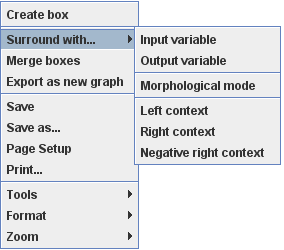
\includegraphics[width=7.5cm]{resources/img/fig5-6b.png}
\caption{Menu contextuel\label{contextual-menu}}
\end{center}
\end{figure}

%%%%%%%%%%%%%%%%%%%%%%%%


\subsection{Sous-graphes}
\label{section-subgraphs}
\index{Graphe!appel à un sous-graphe}\index{\verb+:+}
Pour faire appel à un sous-graphe, il faut indiquer son nom dans une boîte en le faisant
précéder du caractère \verb+:+. Si vous entrez dans une boîte le texte suivant:

\bigskip
\verb$alpha+:beta+gamma+:E:\greek\delta.grf$

\bigskip
\noindent vous obtiendrez une boîte similaire à celle de la figure~\ref{fig-subgraph-call}:

\medskip
\begin{figure}[h]
\begin{center}
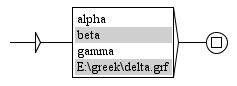
\includegraphics[width=6cm]{resources/img/fig5-7.png}
\caption{Graphe faisant appel aux sous-graphes \texttt{beta} et
\texttt{delta}\label{fig-subgraph-call}}
\end{center}
\end{figure}

\noindent Vous pouvez indiquer le nom complet du graphe
(\verb$E:\greek\delta.grf$) ou simplement le nom sans le chemin d’accès
 (\verb$beta$); dans ce cas, le sous-graphe est supposé se
trouver dans le même répertoire que le graphe qui y fait référence. Il est déconseillé d’utiliser 
des noms de graphes comportant des chemins absolus, car cela nuit à leur portabilité. Si
vous utilisez un nom de graphe absolu, comme c’est ici le cas pour \verb+E:\greek\delta.grf+
le compilateur de graphe émettra un avertissement (voir
figure~\ref{fig-warning-absolute-graph-name}).

\begin{figure}[!h]
\begin{center}
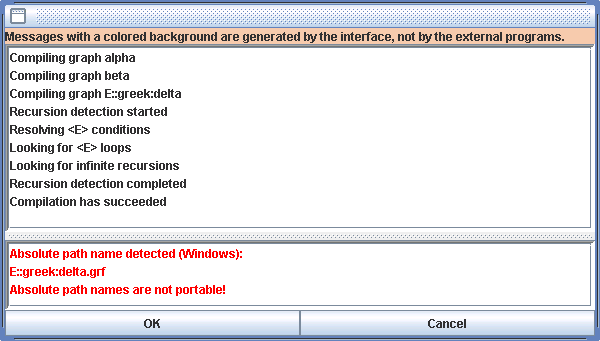
\includegraphics[width=14.5cm]{resources/img/fig5-8.png}
\caption{Avertissement pour un nom de graphe non portable\label{fig-warning-absolute-graph-name}}
\end{center}
\end{figure}


\bigskip
\noindent Pour les mêmes raisons de portabilité, il est déconseillé d’utiliser \verb+\+
ou \verb+/+ comme séparateur dans les noms de graphes. À la place, il vaut mieux utiliser
le caractère \verb+:+ qui joue le rôle de séparateur universel, valable quel que soit le système 
sous lequel vous travaillez. On peut d’ailleurs voir sur la figure
~\ref{fig-warning-absolute-graph-name}
que c’est ce séparateur qui est utilisé en interne par le compilateur de graphe
(\verb+E::greek:delta.grf+).

\bigskip
\noindent \textbf{Répertoire de dépôt}
\label{section-repository}

\bigskip
\noindent Lorsqu’on souhaite réutiliser une grammaire $X$ dans une grammaire $Y$, la méthode
usuelle est de recopier tous les graphes de $X$ dans le répertoire où se trouvent les graphes
de $Y$, ce qui pose deux problèmes :

\begin{itemize}
  \item le nombre de graphes dans le répertoire devient vite très important;
  \item deux graphes ne peuvent pas avoir le même nom.
\end{itemize}

\bigskip
\noindent Afin d’éviter cela, il est possible de stocker la grammaire $X$ dans un répertoire
particulier, appelé \textit{répertoire de dépôt}.\index{Répertoire de dépôt} Ce répertoire est
une sorte de bibliothèque dans laquelle on peut ranger des graphes, et faire ensuite appel
à ces graphes au moyen de \verb+::+  au lieu de \verb+:+. Pour utiliser ce mécanisme, il faut tout
d’abord définir le répertoire de dépôt dans le menu "Info>Preferences...>Directories" (voir figure
	\ref{directories}).
Choisissez votre répertoire dans le cadre "Graph repository". Le répertoire de dépôt est propre
à la langue de travail, vous n’êtes donc pas obligé d’utiliser le même répertoire pour plusieurs
langues.


\begin{figure}[!h]
\begin{center}
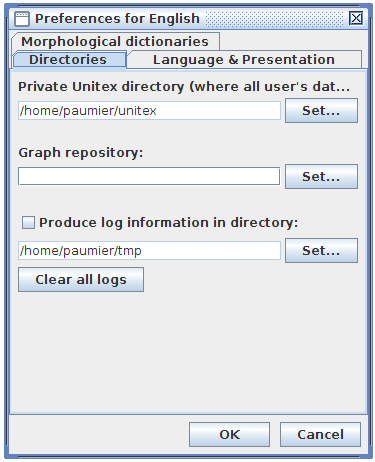
\includegraphics[width=8cm]{resources/img/fig5-10.png}
\caption{Configuration du répertoire de dépôt\label{directories}}
\end{center}
\end{figure}

\bigskip
\noindent Supposons que l’on ait une arborescence comme celle de la figure \ref{repository}. Si l’on
souhaite faire appel au graphe \verb+DET+ qui se trouve dans le sous-répertoire \verb+Johnson+, on
utilisera l’appel

% do not remove this line jump
\noindent \verb+::Det:Johnson:DET+
(voir figure \ref{repository-graph-call}\,\footnote{Dans un souci de clarté, les appels
à des graphes du répertoire de dépôt sont en marron au lieu de gris.}).


\bigskip
\begin{figure}[!h]
\begin{center}
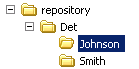
\includegraphics[width=3.9cm]{resources/img/fig5-11.png}
\caption{Exemple de répertoire de dépôt\label{repository}}
\end{center}
\end{figure}

\begin{figure}[!h]
\begin{center}
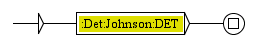
\includegraphics[width=6.7cm]{resources/img/fig5-12.png}
\caption{Appel un graphe du répertoire de dépôt\label{repository-graph-call}}
\end{center}
\end{figure}

\bigskip
\noindent ASTUCE: si vous voulez éviter de mettre dans vos graphes un chemin compliqué
comme \verb+::Det:Johnson:DET+, vous pouvez créer un graphe nommé \verb+DET+ que vous placerez à la
racine du répertoire de dépôt \verb+D:\repository\DET.grf+). Ce graphe contiendra simplement
un appel au graphe \verb+::Det:Johnson:DET+. Vous pourrez alors mettre dans vos graphes un simple
appel à \verb+::DET+. Cela permet 1) de ne pas avoir de noms compliqués et 2) de pouvoir modifier
les graphes du répertoire de dépôt sans avoir à modifier tous vos graphes. En effet, il vous suffira
de mettre à jour le graphe situé à la racine du répertoire de dépôt.

%%%%%%%%%%%%%%%%%%%%%%%%%%%%%%

\begin{figure}[h!]
\begin{center}
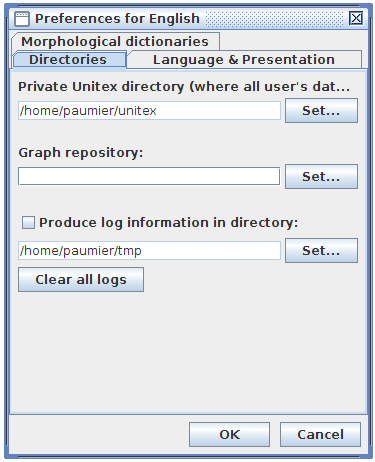
\includegraphics[width=7cm]{resources/img/fig5-9.png}
\caption{Les sous-graphes manquants apparaissent en rouge}
\end{center}
\end{figure}

%%%%%%%%%%%%%%%%%%%%%%%%%%%%

\bigskip
\noindent Les appels à des sous-graphes sont représentés dans les boîtes par des lignes dont
l’arrière-plan est soit gris, soit marron dans le cas de sous-graphes à rechercher dans le 
répertoire de dépôt. Si le fichier \verb+.grf+ du sous-graphe n'est pas trouvé au chemin indiqué,
Unitex cherchera le fichier \verb+.fst2+ de même nom. Si Unitex ne trouve ni le fichier \verb+.grf+
ni le fichier \verb+.fst2+, l'appel au graphe manquant apparaît sur fond rouge. Sous Windows, vous
pouvez ouvrir un sous-graphe en cliquant sur la ligne grisée tout en appuyant sur la touche Alt.
Sous Linux, la combinaison <Alt+Click> est interceptée par le système\footnote{Si vous travaillez
sous KDE, désactivez <Alt+Click> dans kcontrol.} :
pour ouvrir un sous-graphe, faites un clic central sur son nom (avec le bouton central) ou faites un clic simultané (avec les boutons gauche
et droit).

%%%%%%%%%%%%%%%%%%%%

\bigskip
\noindent La liste des graphes appelés par le graphe courant et celle des graphes qui appellent le
graphe courant peuvent être affichées en cliquant sur le second et troisième bouton du quatrième
groupe de boutons de la barre d'outils (voir figure~\ref{list-called-graphs} et
figure~\ref{fig-toolbar} à la section~\ref{toolbar-commands}).
Dans ces listes de sous-graphes:
\begin{itemize}
\item les sous-graphes directement appelés par le graphe courant apparaissent avec leur simple nom
	de fichier
\item les sous-graphes indirectement appelés par l'un des graphes appelés par le graphe courant
	apparaissent avec une flèche devant leurs nom
\item les sous-graphes qui apparaissent dans des graphes appelés par le graphe courant sans être
	connectés et donc non traités  ont leur nom en orange
\item les sous-graphes non trouvés (ni en .grf ni en .fst2) apparaissent en rouge.
\end{itemize}

\begin{figure}[!h]
\begin{center}
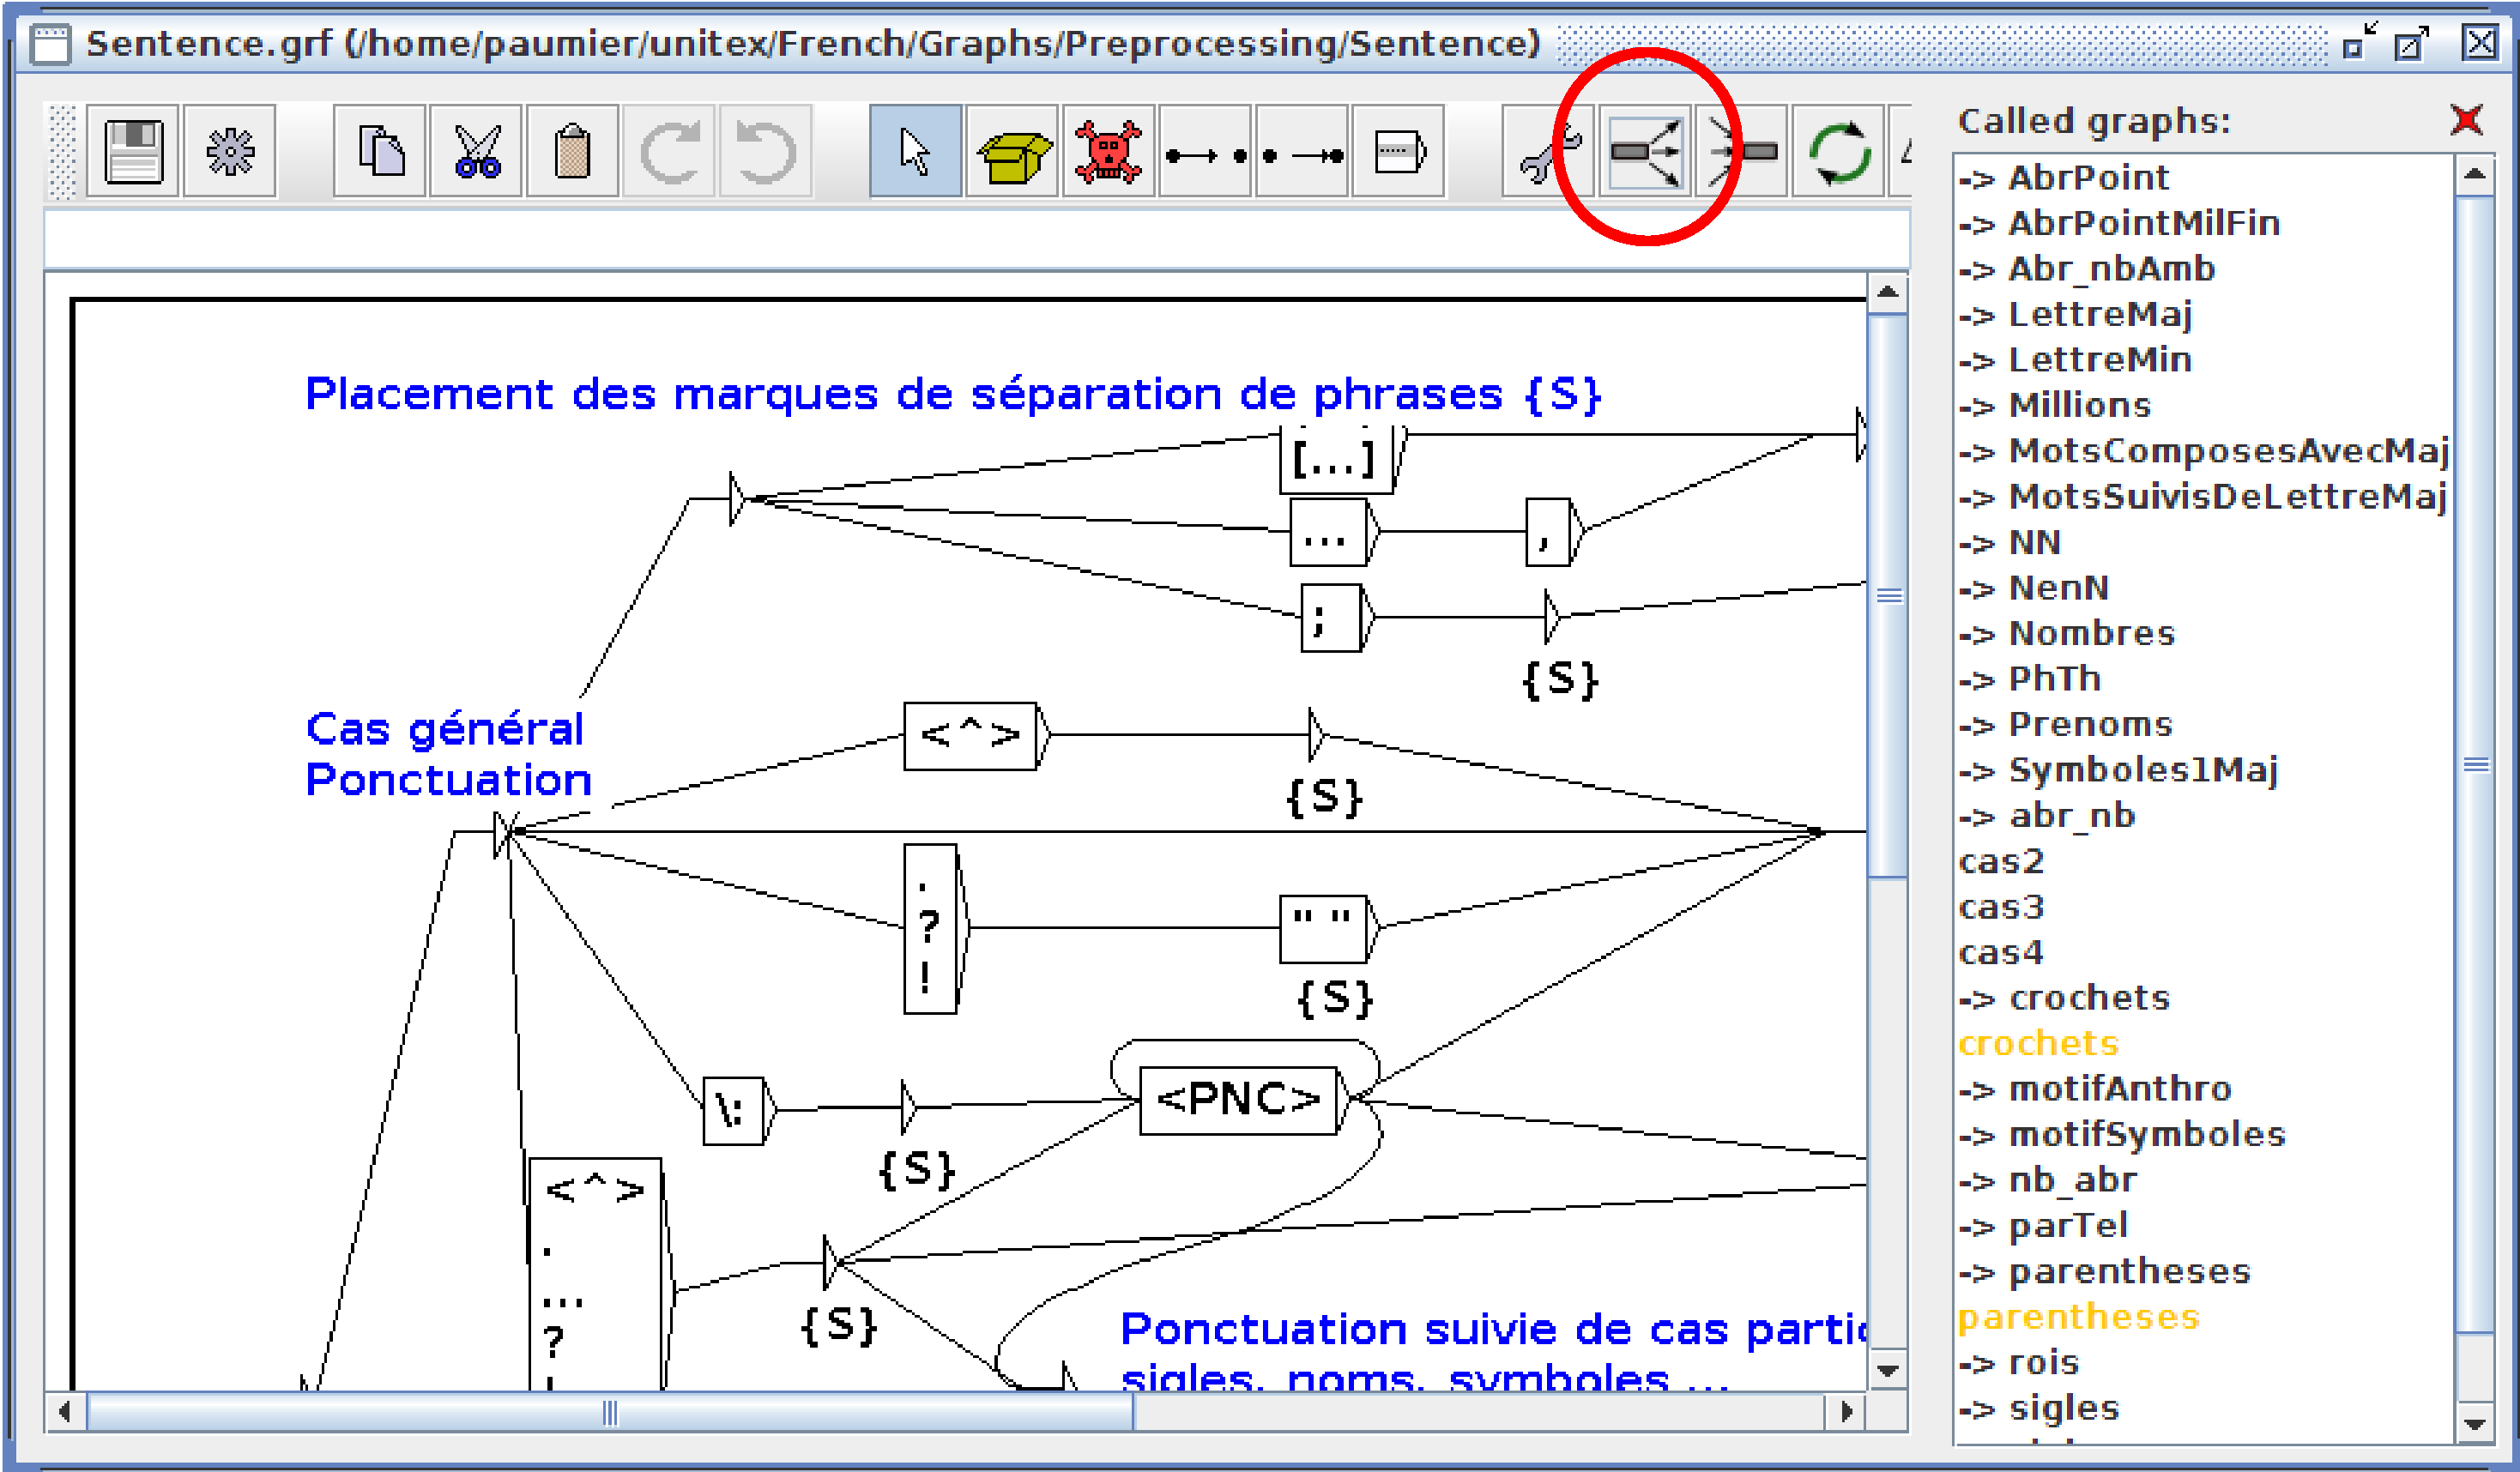
\includegraphics[width=15.2cm]{resources/img/fig5-12b.png}
\caption{Affichage de la liste de tous les graphes appelés\label{list-called-graphs}}
\end{center}
\end{figure}


%%%%%%%%%%%%%%%%%%

\subsection{Manipulation des boîtes}
\index{Sélection multiple}\index{Boîtes!sélection}

Vous pouvez sélectionner plusieurs boîtes au moyen de la souris. Pour cela, cliquez et
déplacez la souris sans relâcher le bouton. Lorsque vous relâcherez le bouton, toutes les
boîtes touchées par le rectangle de sélection seront sélectionnées et s’afficheront alors en
blanc sur fond bleu, figure \ref{multi-selection}.

\begin{figure}[!ht]
\begin{center}
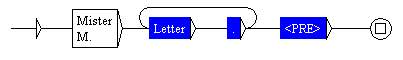
\includegraphics[width=10cm]{resources/img/fig5-13.png}
\caption{Sélection de plusieurs boîtes\label{multi-selection}}
\end{center}
\end{figure}
\vspace{-0.3cm}
%%%%%%%%%%%%%%%
%\bigskip
\noindent Vous pouvez sélectionner plusieurs boîtes en maintenant les touches <CTRL> et <SHIFT> et
en cliquant sur chaque boîte à ajouter à la sélection. De cette manière, vous pouvez sélectionner
plusieurs boîtes sans avoir à sélectionner une zone complète.

\begin{figure}[!ht]
\begin{center}
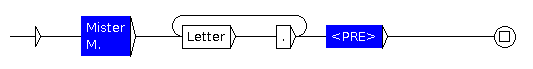
\includegraphics[width=10cm]{resources/img/fig5-13b.png}
\caption{Sélection de boîtes éloignées\label{multi-selection2}}
\end{center}
\end{figure}
\vspace{-0.3cm}


%%%%%%%%%%%%%%
\bigskip
\noindent Lorsque des boîtes sont sélectionnées, vous pouvez les déplacer en cliquant et en déplaçant le curseur sans relâcher le bouton. Pour annuler la sélection, cliquez sur une zone vide
du graphe ; si vous cliquez sur une boîte, toutes les boîtes de la sélection seront reliées à
celle-ci.

\bigskip
\index{Sélection multiple!copier-coller}
\index{Copier}\index{Coller}
\noindent Vous pouvez effectuer un copier-coller sur plusieurs boîtes. Pour cela, sélectionnez-les
et appuyez sur <Ctrl+C> ou cliquez sur "Copy" dans le menu "Edit". Votre sélection multiple
est maintenant dans le presse-papiers d’Unitex. Vous pouvez alors coller cette sélection en
pressant <Ctrl+V> ou en cliquant sur "Paste" dans le menu "Edit".


\bigskip
\begin{figure}[!h]
\begin{center}
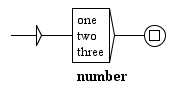
\includegraphics[width=13cm]{resources/img/fig5-14.png}
\caption{Copier-coller d’une sélection multiple}
\end{center}
\end{figure}

\noindent NOTE: Vous pouvez coller une sélection multiple dans des graphes différents de celui dont
elle est issue.

\bigskip
\index{Graphes!suppression de boîtes}\index{Boîtes!suppression}
\noindent Pour supprimer des boîtes, sélectionnez-les, effacez le texte qu'elles contiennent
(\textit{i.e.} le texte affiché dans le champ situé en haut de la fenêtre)
 et appuyez sur Enter. L'état initial et l'état final ne peuvent être supprimés.

\subsection{Sortie}
\index{Transducteurs}\index{\verb+/+}
Il est possible d’associer une sortie à une boîte. Pour cela, utilisez le caractère spécial
\verb+/+. Tous les caractères situés à droite de celui-ci seront considérés comme faisant partie de
la sortie. Ainsi, le texte \verb$one+two+three/number$ donne la boîte de la figure
~\ref{fig-exemple-transduction}. La sortie associée à une boîte est représentée en texte gras
sous celle-ci.\\


%\bigskip
\begin{figure}[h]
\begin{center}
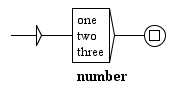
\includegraphics[width=4.5cm]{resources/img/fig5-15.png}
\caption{Exemple de sortie\label{fig-exemple-transduction}}
\end{center}
\end{figure}


%%%%%%%%%%%%%%
\noindent \textbf{Poids}\\


Vous pouvez attribuer des poids à des boîtes d'un transducteur. Ainsi, lorsqu'une séquence est
reconnue par plusieurs chemins, seul celui de poids le plus élévé sera conservé.
Après un "Locate", la concordance, ne comportera qu'une seule fois la séquence reconnue avec la
sortie appropiée (figure~\ref{fig-weights-in-graphs}).

\bigskip
\begin{figure}[h!]
\begin{center}
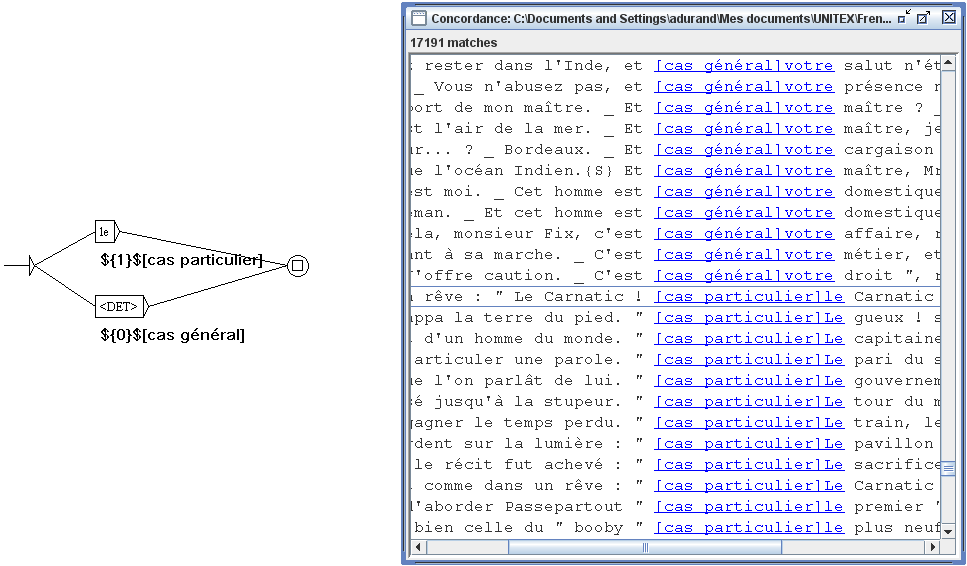
\includegraphics[width=14.5cm]{resources/img/fig5-15b.png}
\caption{Poids dans les graphes \label{fig-weights-in-graphs}}
\end{center}
\end{figure}

%%%%%%%%%%%%%

\subsection{Utilisation des variables}
\label{section-using-variables}
\index{Graphe!variables}\index{Variables!dans les graphes}\index{\verb+$+}
\index{Transducteur!avec variables}

Il est possible de sélectionner des parties du texte reconnu par une grammaire au moyen
de variables. Pour associer une variable \verb+var1+ à une partie d’une grammaire, utilisez
les symboles spéciaux \verb+$var1(+ et \verb+$var1)+ pour définir respectivement le début et
la fin de la zone à stocker. Créez deux boîtes contenant l’une \verb+$var1(+ et l’autre
\verb+$var1)+. Ces boîtes ne doivent rien contenir d’autre que le nom de la variable précédé de
 \verb+$+ et suivi d’une parenthèse. Reliez ensuite ces boîtes à la zone de la grammaire voulue.
 Dans le graphe de la figure ~\ref{fig-using-variable} on reconnaît une séquence commençant par
 un nombre que l’on stocke dans une variable nommée \verb+var1+, suivi de \verb+dollar+ ou
 \verb+dollars+.

\bigskip
\begin{figure}[h]
\begin{center}
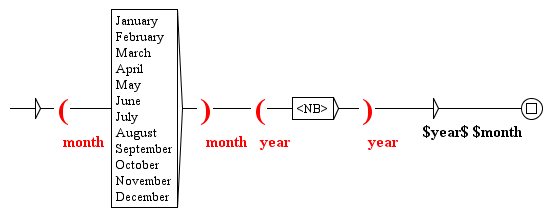
\includegraphics[width=13.5cm]{resources/img/fig5-16.png}
\caption{Utilisation d’une variable
\texttt{var1}\label{fig-using-variable}}
\end{center}
\end{figure}

\noindent Les noms de variables peuvent contenir des lettres latines non accentuées, minuscules
ou majuscules, ainsi que des chiffres et le caractère \verb+_+ (underscore).
\index{\verb+_+}\index{Noms de variables} Unitex fait la différence entre les lettres minuscules
et majuscules.\index{Underscore}

\bigskip
\noindent Quand une variable a ainsi été définie, on peut l’utiliser dans les sorties en encadrant
son nom avec le caractère \verb+$+.\index{\verb+$+} La grammaire de la figure
~\ref{fig-date-grammar} reconnaît une date formée d’un mois et d’une année,
 et produit en sortie la même date, mais dans l’ordre année-mois.

%Si l’on souhaite écrire en sortie le caractère \verb+$+.
%il faut le doubler, comme c’est le cas dans la figure ~\ref{fig-using-variable}.
\noindent Si vous voulez utiliser le caractère \verb+$+ en sortie d'une boîte, vous devez le
redoubler, comme le montre la figure~\ref{fig-using-variable}.

\bigskip
\begin{figure}[h]
\begin{center}
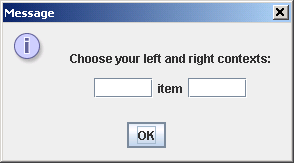
\includegraphics[width=14.5cm]{resources/img/fig5-17.png}
\caption{Inversion du mois et de l’année dans une date\label{fig-date-grammar}}
\end{center}
\end{figure}

%\noindent Si vous voulez utiliser le caractère \verb+$+ en sortie d'une boîte, vous devez le
%redoubler, comme le montre la figure~\ref{fig-using-variable}.

\bigskip
\noindent Par défaut \verb+Locate+ et \verb+LocateTfst+ considèrent que les variables non définies
sont vides. Vous pouvez modifier ce comportement (voir section \ref{section-advanced-search-options}).
De plus, il est  possible de savoir si une variable est définie ou non (voir section
\ref{section-variables}).

\subsection{Copie de listes}
\index{Copie de listes}
\index{Copie}\index{Coller}

Il peut être pratique d’effectuer un copier-coller d’une liste de mots ou d’expressions
depuis un éditeur de texte vers une boîte dans un graphe. Afin d’éviter de devoir copier
manuellement chaque terme, Unitex propose un mécanisme de copie de listes. Pour l’utili-
ser, sélectionnez votre liste dans votre éditeur de texte et copiez-la au moyen de <Ctrl+C> ou
de la fonction de copie intégrée à votre éditeur. Créez ensuite une boîte dans votre graphe,
et utilisez <Ctrl+V> ou la commande "Paste" du menu "Edit" pour la coller dans la boîte.
Vous verrez alors apparaître la fenêtre de la figure~\ref{fig-setting-contexts-for-multiple-copy}:

\bigskip
\begin{figure}[h]
\begin{center}
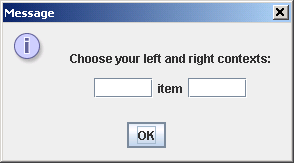
\includegraphics[width=7cm]{resources/img/fig5-18.png}
\caption{Sélection de contexte pour la copie d’une
liste\label{fig-setting-contexts-for-multiple-copy}}
\end{center}
\end{figure}
\index{Contextes!copie de liste}

\noindent Cette fenêtre vous permet de définir les contextes gauche et droit qui seront ajoutés
automatiquement à chaque terme de la liste. Par défaut, ces contextes sont vides. Si l’on applique
les contextes \verb+<+ et \verb+.V>+ à la liste suivante:

\bigskip
\textit{eat}

\textit{sleep}

\textit{drink}

\textit{play}

\textit{read}

\bigskip
\noindent on obtient la boîte de la figure~\ref{fig-multiple-copy}:

\bigskip
\begin{figure}[h]
\begin{center}
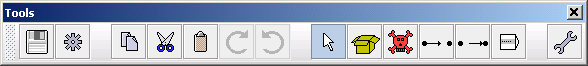
\includegraphics[width=6.7cm]{resources/img/fig5-19.png}
\caption{Boîte obtenue par copie d’une liste avec ajout de contextes\label{fig-multiple-copy}}
\end{center}
\end{figure}

\subsection{Symboles spéciaux}
\index{Symboles!spéciaux}
\noindent L’éditeur de graphes d’Unitex interprète de façon particulière les symboles suivants:

\bigskip
\verb," + : / < > # \,

\bigskip
\noindent Le tableau ~\ref{tab-special-symbols} résume la signification pour Unitex de ces symboles,
ainsi que la ou les façons de reconnaître ces caractères dans des textes.


\bigskip
\index{Meta-caractères}
\begin{table}[h]
\begin{center}
\begin{tabular}{|c|p{9cm}|c|}
\hline
\texttt{Caractère} & \texttt{Signification} & \texttt{Codage}
\\
\hline \verb$"$ & les guillemets délimitent des séquences qui ne doivent
ni être interprétées par Unitex, ni subir de variantes de casse
& \verb$\"$
\\
\hline
\verb$+$ & \verb$+$ sépare les différentes lignes boîtes& \verb$"+"$
\\
\hline
\verb$:$ & \verb$:$ sert à introduire à appel à un sous-graphe& \verb$":"$ or \verb$\:$
\\
\hline
\verb$/$ & \verb$/$ indique le début de la sortie d'une boîte& \verb$\/$
\\
\hline
\verb$<$ & \verb$<$ indique le début d'un motif ou d'un méta& \verb$"<"$ or \verb$\<$
\\
\hline
\verb$>$ & \verb$>$ indique la fin d'un motif ou d'un méta& \verb$">"$ or \verb$\>$
\\
\hline
\verb$#$ & \verb$#$ sert à interdire la présence de l'espace& \verb$"#"$
\\
\hline
\verb$\$ & \verb$\$ sert à déspécialiser la plupart des caractères spéciaux& \verb$\\$
\\
\hline
\end{tabular}
\caption{Codage des symboles spéciaux dans l’éditeur de graphes\label{tab-special-symbols}}
\end{center}
\end{table}

\subsection{Commandes de la barre d’icônes}
\index{Barre d'outils}
\label{toolbar-commands}

La barre d’icônes présente au-dessus des graphes contient des raccourcis vers certaines
commandes et permet de manipuler les boîtes d’un graphe en utilisant des "outils". Cette
barre d’icônes peut être déplacée en cliquant sur la zone "rugueuse". Elle peut même être
dissociée du graphe et apparaître alors comme une fenêtre séparée (voir figure~\ref{fig-toolbar}).
Dans ce cas, le fait de fermer cette fenêtre replace la barre d’icônes à sa position initiale.
Chaque graphe possède sa propre barre d’icônes.
\vspace{-0.1cm}
\begin{figure}[!ht]
\begin{center}
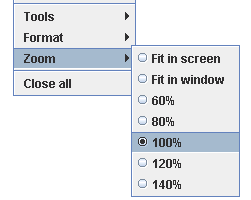
\includegraphics[width=15cm]{resources/img/fig5-20.png}
\caption{Barre d'outils\label{fig-toolbar}}
\end{center}
\end{figure}
\index{Copy}\index{Cut}\index{Paste}
\vspace{-0.3cm}

%\bigskip
\noindent Les deux premières icônes sont des raccourcis permettant de sauver et de compiler le
graphe. Les cinq suivantes correspondent aux opérations "Copier", "Couper", "Coller", "Redo" et
"Undo".\\

Les 6 icônes suivantes correspondent à des commandes d’édition des boîtes. La première,
en forme de flèche blanche, correspond au mode d’édition normal des boîtes. Les 5 autres
correspondent à des outils. Pour utiliser un outil, cliquez sur l’icône correspondante : le
curseur de la souris changera alors de forme et les clics de la souris seront alors interprétés
de façon particulière. Voici la description des outils, de gauche à droite:

\begin{itemize}
  \item création de boîtes: crée une boîte vide à l’endroit du clic;
  \item suppression de boîtes: supprime la boîte sur laquelle vous cliquez;
  \item relier des boîtes à une autre boîte: cet outil permet de sélectionner une ou plusieurs
boîtes, et de la ou les relier à une autre. À la différence du mode normal, la ou les
transitions qui vont être créées sont affichées pendant le déplacement du pointeur de
la souris;
  \item relier des boîtes à une autre boîte en sens inverse: cet outil effectue la même chose que
le précédent, mais en reliant en sens inverse les boîtes sélectionnées à la boîte cliquée;
  \item ouvrir un sous-graphe: ouvre un sous-graphe lorsque vous cliquez sur la ligne grisée
correspondante dans une boîte.
\end{itemize}

L'icône en forme de clé est un raccourci pour ouvrir la fenêtre des options d'affichage
du graphe. Les deux suivantes permettent de voir les listes de graphes en relation avec le
graphe courant:

\begin{itemize}
\item Le premier bouton affiche la liste des graphes appelés par le graphe courant
\item Le seconde bouton affiche la liste des graphes qui appellent le graphe courant
\end{itemize}

Le bouton muni de deux flèches vertes rafraîchit le graphe courant en chargeant sa dernière version.
Si un fichier \verb+.grf+ est modifié alors que le graphe qu'il contient est affiché dans
une fenêtre Unitex, une fenêtre pop up vous invitera à le recharger.

\bigskip
\noindent Le bouton portant l'icone d'une balance permet de comparer le graphe courant à un autre
graphe ou à une autre version du même graphe. Une nouvelle fenêtre est alors affichée (voir
	figure~\ref{Graph-DIFF}) qui contient les deux graphes avec des couleurs qui mettent en
relief les types de différences qui existent entre les deux graphes : insertion, suppression,
déplacement de boîtes et changement de contenu d'une boîte apparaissent respectivement en vert,
rouge, mauve et jaune.

\bigskip
\noindent 
\begin{figure}[!h]
\begin{center}
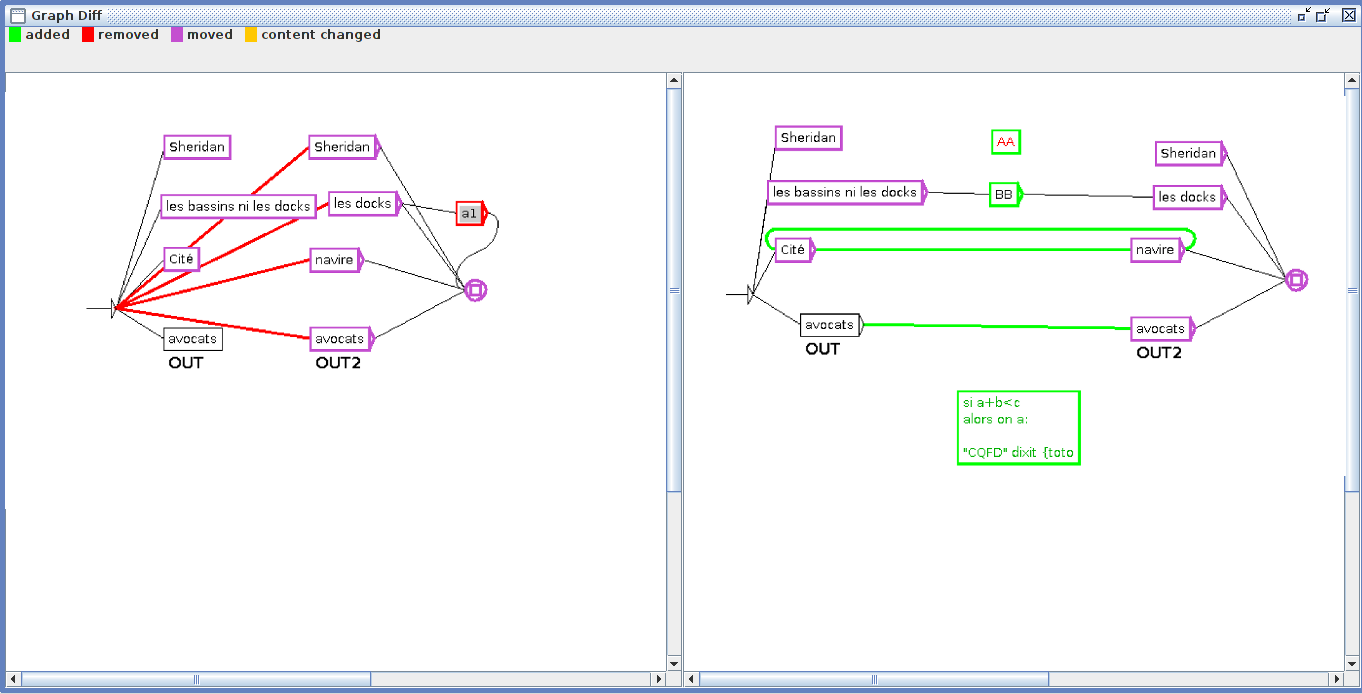
\includegraphics[width=15.6cm]{resources/img/DIFF.png}
\caption{DIFF\label{Graph-DIFF}}
\end{center}
\end{figure}
\bigskip
\noindent

Les six derniers boutons sont des raccourcis pour l'utilisation des variables, du mode morphologique
ou l'ajout de contextes autour d'une ou plusieurs boîtes sélectionnées. Ces boutons ne sont activés que si une  ou plusieurs boîtes sont sélectionnées:
\begin{itemize}
\item \textcolor{red}{()}  : variable normale	(voir section~\ref{section-using-variables})
\item \textcolor{blue}{()} : variable de sortie (voir section~\ref{section-output-variables})
\item \textcolor{magenta}{<>} : mode morphologique (voir section~\ref{section-morphological-mode})
\item \textcolor{green}{\$*} : contexte gauche (voir section~\ref{section-contexts})
\item \textcolor{green}{\$[} : contexte droit (voir section~\ref{section-contexts})
\item \textcolor{green}{\$![} : contexte droit négatif (voir section~\ref{section-contexts})
\end{itemize}

\bigskip
%\pagebreak


%%%%%%%%%%%%%%%%%%%

\section{Options de présentation}
\index{Graphe!présentation}

\subsection{Tri des lignes d’une boîte}
\index{Tri!des lignes d'une boîtes}\index{Boîtes!tri des lignes}
Vous pouvez trier le contenu d’une boîte en la sélectionnant et en cliquant sur "Sort Node
Label" dans le sous-menu "Tools" du menu "FSGraph". Ce tri ne fait pas appel au programme
\verb+SortTxt+. Il s’agit d’un tri basique qui trie les lignes de la boîte selon l’ordre des
caractères dans le codage Unicode.\index{Unicode}


\subsection{Zoom}
\index{Zoom}\index{Graphe!zoom}
Le sous-menu "Zoom" vous permet de choisir l’échelle à laquelle sera affiché le graphe.

\bigskip
\begin{figure}[h]
\begin{center}
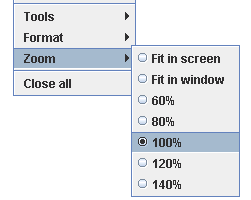
\includegraphics[width=6.4cm]{resources/img/fig5-21.png}
\caption{Sous-menu Zoom}
\end{center}
\end{figure}

\noindent L’option "Fit in screen" étire ou rétrécit le graphe pour lui donner la taille de l’écran.
L’option "Fit in window" ajuste le graphe pour qu’il soit entièrement affiché dans la fenêtre.


\subsection{Antialiasing}
\index{Antialiasing}\index{Graphe!antialiasing}
L’antialiasing est un effet de rendu qui permet d’éviter l’effet de pixellisation.
\index{Pixellisation} Vous pouvez activer cet effet en cliquant sur "Antialiasing..."
dans le sous-menu "Format". La figure~\ref{fig-antialiasing} montre deux graphes affichés
normalement (graphe du haut) et avec antialiasing (graphe du bas).


\bigskip
\begin{figure}[!ht]
\begin{center}
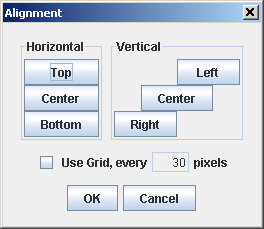
\includegraphics[width=13.5cm]{resources/img/fig5-22.png}
\caption{Exemple d'antialiasing\label{fig-antialiasing}}
\end{center}
\end{figure}

\noindent Cet effet ralentit l’exécution d’Unitex. Nous vous conseillons de ne pas l’utiliser
si votre machine est peu puissante.


%\clearpage

\subsection{Alignement des boîtes}\index{Boîtes!alignement}
\index{Alignement des boîtes}\index{Graphe!alignement des boîtes}
Afin d’obtenir des graphes harmonieux, il est utile de pouvoir aligner les boîtes, aussi
bien horizontalement que verticalement. Pour cela, sélectionnez les boîtes à aligner et cli-
quez sur "Alignment..." dans le sous-menu "Format" du menu "FSGraph" ou appuyez sur
<Ctrl+M>. Vous voyez alors apparaître la fenêtre de la figure~\ref{fig-alignment-frame}.

\bigskip
\noindent Les possibilités d’alignement horizontal sont:
\begin{itemize}
  \item Top: les boîtes sont alignées sur la boîte la plus haute;
  \item Center: les boîtes sont toutes centrées sur un même axe;
  \item Bottom: les boîtes sont alignées sur la boîte la plus basse.
\end{itemize}

\begin{figure}[!h]
\begin{center}
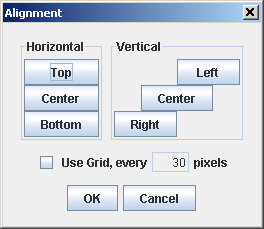
\includegraphics[width=6.6cm]{resources/img/fig5-23.png}
\caption{Fenêtre d’alignement\label{fig-alignment-frame}}
\end{center}
\end{figure}

\noindent Les possibilités d’alignement vertical sont:
\begin{itemize}
  \item Left: les boîtes sont alignées sur la boîte la plus à gauche;
  \item Center: les boîtes sont toutes centrées sur un même axe;
  \item Right: les boîtes sont alignées sur la boîte la plus à droite.
\end{itemize}

\bigskip
\noindent La figure ~\ref{fig-vertical-left-alignment} montre un exemple 
d’alignement. Le groupe de boîtes situé à droite est une copie des boîtes
de gauche qui a été alignée verticalement à gauche.


\bigskip
\begin{figure}[!h]
\begin{center}
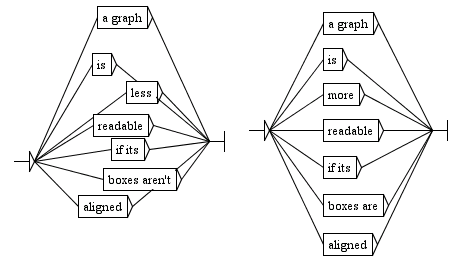
\includegraphics[width=11.5cm]{resources/img/fig5-24.png}
\caption{Exemple d’alignement vertical gauche\label{fig-vertical-left-alignment}}
\end{center}
\end{figure}

\bigskip
\noindent L’option "Use Grid" de la fenêtre d’alignement permet d’afficher une grille en
arrière-plan du graphe. Cela permet d’aligner approximativement les boîtes.
\index{Grille}

\bigskip
\begin{figure}[!h]
\begin{center}
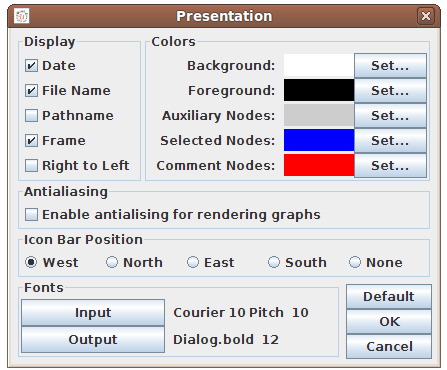
\includegraphics[width=15cm]{resources/img/fig5-25.png}
\caption{Exemple d’utilisation d’une grille}
\end{center}
\end{figure}

\subsection{Présentation, polices et couleurs}
\label{section-display-fonts-colors}
\index{Graphe!options d'affichage, polices et couleurs}\index{Options!configuration}
\index{Couleurs!configuration}
Vous pouvez configurer l’aspect d’un graphe en appuyant sur <Ctrl+R> ou en cliquant
sur "Presentation..." dans le sous-menu "Format" du menu "FSGraph", ce qui provoque l’af-
fichage de la fenêtre de la figure~\ref{fig-graph-display-configuration}.

\begin{figure}[!h]
\begin{center}
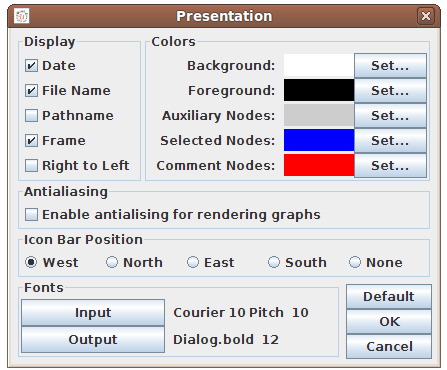
\includegraphics[width=9cm]{resources/img/fig5-26.png}
\caption{Configuration de l’aspect d’un graphe\label{fig-graph-display-configuration}}
\end{center}
\end{figure}

\bigskip
\noindent Les paramètres de polices sont:
\begin{itemize}
  \item Input: police utilisée dans les boîtes, ainsi que dans la zone de texte où l’on édite le
contenu des boîtes;
\item Output: police utilisée pour afficher les sorties des boîtes.\index{Sorties d'un transducteur}
\end{itemize}

\bigskip
\noindent Les paramètres de couleur sont:
\begin{itemize}
  \item Background: couleur de fond;
  \item Foreground: couleur utilisée pour le texte et le dessin des boîtes;
  \item Auxiliary Nodes: couleur des boîtes faisant appel à des sous-graphes ;
  \item Selected Nodes: couleur utilisée pour dessiner les boîtes quand elles sont sélectionnées ;
  \item Comment Nodes: couleur utilisée pour dessiner les boîtes qui ne sont reliées à aucune autre.
\end{itemize}

\bigskip
\noindent Les autres paramètres sont:
\begin{itemize}
  \item Date: affichage de la date courante dans le coin inférieur gauche du graphe;
  \item File Name: affichage du nom du graphe dans le coin inférieur gauche du graphe;
  \item Pathname: affichage du nom du graphe avec son chemin complet dans le coin inférieur
gauche du graphe. Cette option n’a d’effet que si l’option "File Name" est sélectionnée;
  \item Frame: dessine un cadre autour du graphe;
  \item Right to Left: inverse le sens de lecture du graphe (voir exemple de la
  		  figure~\ref{fig-right-to-left-graph}).
\end{itemize}

\bigskip
\begin{figure}[!h]
\begin{center}
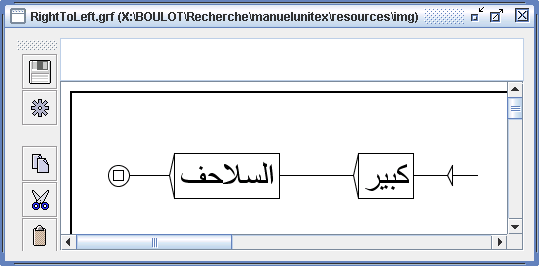
\includegraphics[width=14.5cm]{resources/img/fig5-27.png}
\caption{Graphe se lisant de droite à gauche\label{fig-right-to-left-graph}}
\end{center}
\end{figure}

\bigskip
\noindent Vous pouvez rétablir les paramètres par défaut en cliquant sur le bouton "Default".
Si vous cliquez sur le bouton "OK", seul le graphe courant sera modifié.\index{Preferences}
Pour modifier les préférences par défaut d’une langue, cliquez sur "Preferences..." dans le
menu "Info" et choisissez l’onglet "Graph Presentation".

%La fenêtre de configuration des préférences possède
%une option supplémentaire concernant l’antialiasing (voir figure
%order to modify the preferences for a language as a default, click on
%"Preferences..." in the "Info" menu and click on the "Graph configuration" button 
%in the "Language \& Presentation" tab.


\section{Les graphes en dehors d’Unitex}
\subsection{Inclusion d’un graphe dans un document}
\index{Graphe!inclure dans un document}\index{Inclure un graphe dans un document}
\index{Graphe!export en PNG}
Pour inclure un graphe dans un document, il faut en faire une image. Pour cela, une
première méthode consiste à sauver votre graphe en tant qu’image au format PNG. Pour
cela, allez dans le menu "FSGraph" et cliquez sur "Save as...". Choisissez ensuite le type de
fichier PNG. Vous obtiendrez ainsi une image prête à être intégrée dans un document ou
à être éditée avec un logiciel de retouche d’images. Afin de rendre l’image plus lisse, vous
pouvez activer l’antialiasing pour le graphe qui vous intéresse.


\bigskip
\noindent La seconde méthode consiste à faire une capture d’écran:

\bigskip
\noindent Sous Windows:

\bigskip
\noindent Appuyez ensuite sur la touche "Imprime écran" de votre clavier qui doit se trouver près
de la touche F12. Lancez le programme \verb+Paint+ dans le menu "Accessoires" de Windows. Appuyez sur 
<Ctrl+V>. \verb+Paint+ devrait vous dire que l’image contenue dans le presse-papiers
est trop grande et vous demander si vous voulez agrandir l’image. Cliquez sur "Oui". Vous
pouvez maintenant éditer l’image de l’écran. Sélectionnez la zone qui vous intéresse. Pour
cela, passez en mode sélection en cliquant sur le rectangle en pointillé qui se trouve dans
le coin supérieur gauche de la fenêtre. Vous pouvez maintenant sélectionner une zone de
l’image avec la souris. Une fois votre zone sélectionnée, appuyez sur <Ctrl+C>. Votre sélection
est maintenant dans le presse-papier, il ne vous reste plus qu’à aller dans votre document
et à appuyer sur <Ctrl+V> pour coller votre image.


\bigskip
\noindent Sous Linux:

\bigskip
\noindent Effectuez une capture d’écran (par exemple avec le programme \verb+xv+). Retaillez ensuite
votre image avec un éditeur graphique (par exemple \verb+TheGimp+), et collez votre image dans
votre document de la même façon que sous Windows.


\newpage
\bigskip
\noindent\textbf{Vector graphics}
\index{SVG export de graphe}
\index{Graphe!export SVG}

\bigskip
\noindent Si vous préférez vector graphics, vous pouvez enregistrer votre graphe en format
SVG, qui est utilisable avec des logiciels comme  Inkscape (\cite{Inkscape}).
Il permet d'obtenir des sorties PostScript utilisables dans des documents \LaTeX.

\subsection{Impression d’un graphe}
\index{Impression d’un graphe}\index{Impression!d’un graphe}

Vous pouvez imprimer un graphe en cliquant sur "Print..." dans le menu "FSGraph" ou
en appuyant sur <Ctrl+P>.


\bigskip
\noindent ATTENTION: vous devez vous assurer que le paramètre d’orientation de l’imprimante
(portrait ou paysage) correspond bien à l’orientation de votre graphe.


\bigskip
\noindent Vous pouvez définir vos préférences d’impression en cliquant sur "Page Setup" dans le
menu "FSGraph". Vous pouvez également imprimer tous les graphes qui sont ouverts en
cliquant sur "Print All...".



